\chapter{Platform analysis} \label{ch:plaanalysis}
In this chapter the hardware platform provided for this project is described. For this project, HSA systems have provided a Zedboard Development Board \cite{Zedboard2014}. This board is used for this project since it contains a Zynq Z-7020 SoC from Xilinx, which HSA Systems uses for multiple products.

\section{Platform trade-off}
When designing embedded systems the choice of platform is important. Different platform exists each with their own advantages and disadvantages. Figure \vref{fig:plattrade} illustrates the relation between design time and flexibility for some general platform types, inspired by \cite{adams2002choosing}. \\

\begin{figure}[ht!]
  \centering
  %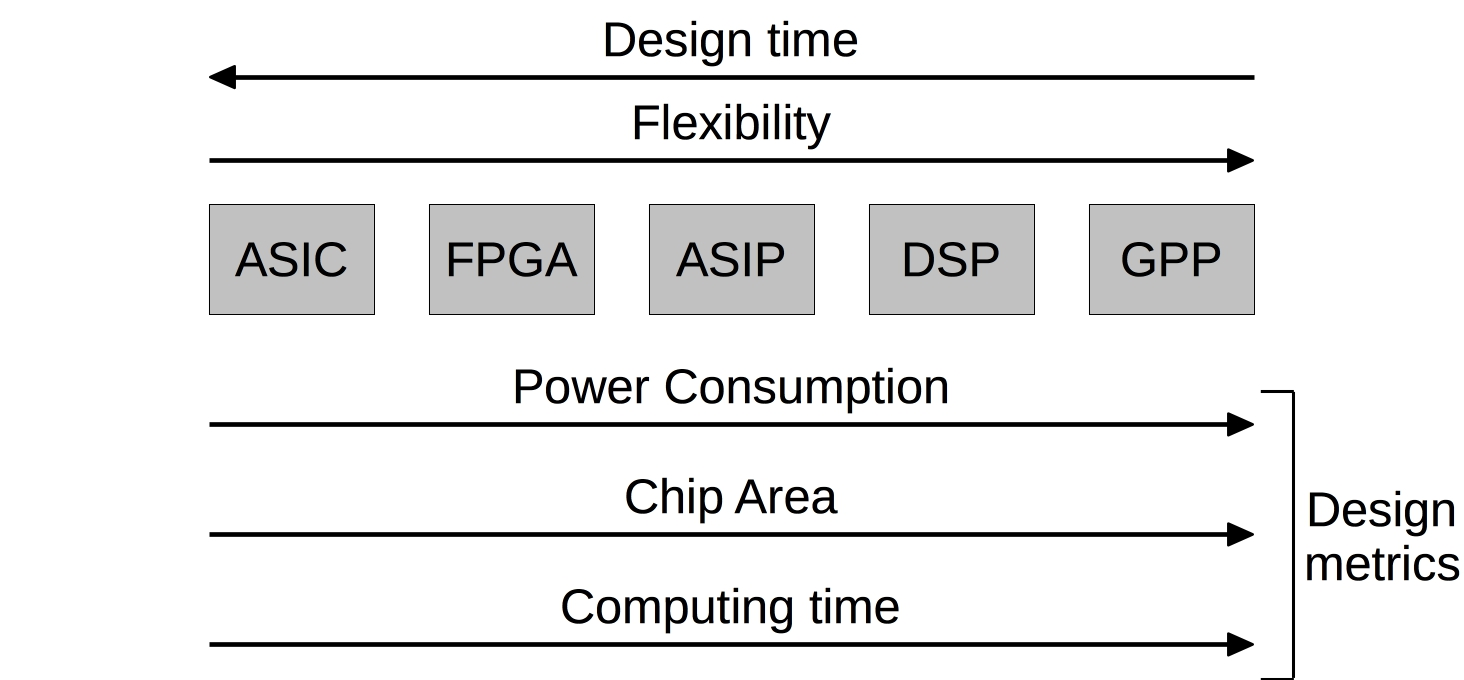
\includegraphics[width=0.7\textwidth]{figures/plattrade2}
  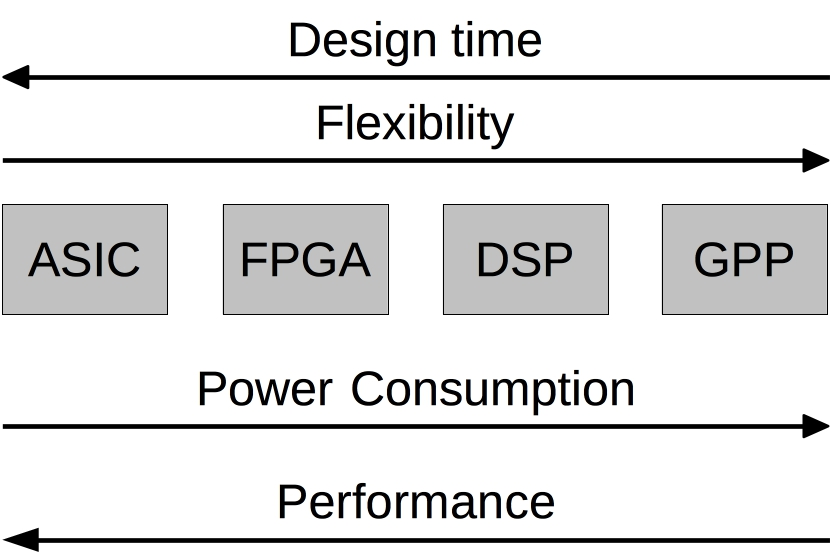
\includegraphics[width=0.4\textwidth]{figures/plattrade3}
  \caption{Relation between design time and flexibility for general platform types.}
  \label{fig:plattrade}
\end{figure}
From figure \vref{fig:plattrade} it is seen that there is a clear trade-off between a general-purpose processor (GPP) and an application specific integrated circuit (ASIC). The other platforms fall in between these two.\\

A GPP is a popular choice due to its short design time and high flexibility. It is optimized for data manipulation, control flow, and sequential performance. However in the area of signal processing applications usually have a high number of computations and a high level of inherent parallelism. This makes a GPP not the best platform for such applications. For these applications, more specialized platforms can be used such as a DSP or FPGA. A DSP includes optimized computational units which can be used for real-time signal processing. But DSPs require the designer to have a better knowledge of the specific DSP platform when designing for it. The DSP is still limited by the number of computational units on the platform. This is where an FPGA is strong. An FPGA consists of a high number of logic gates and interconnections between them and with this specialized architectures can be designed which can completely utilize the inherent parallelism in an algorithm.\\ 

In later years new platforms have emerged which combines some the general platforms. This is clearly seen with platforms such as Zynq Z-7020 which is a GPP combined with an FPGA.\\ 

HSA Systems has chosen that the platform for this project will be a Zedboard which contains a Zynq Z-7020 since this chip is used in other of the company's products. This project will mainly only use the programmable logic of the Zynq SoC since the project description states that the focus is on an FPGA implementation.

\section{Zynq Z-7020}

\begin{figure}[ht!]
  \centering
  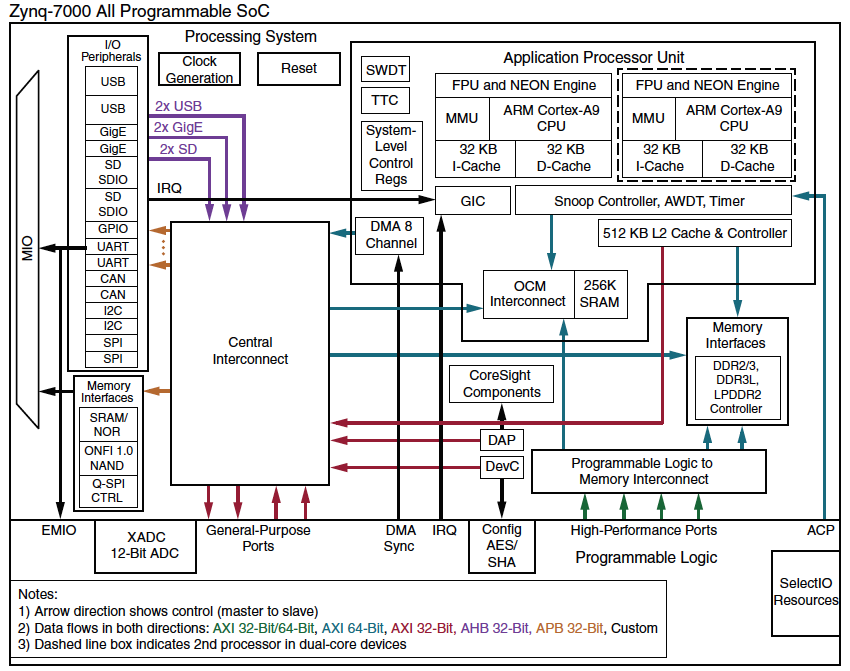
\includegraphics[width=0.75\textwidth]{figures/z7020overview}
  \caption{Architectural Overview \cite{zynq20137000}}
  \label{fig:z7020over}
\end{figure}

The Zynq SoC contains an ARM$^\text{\textregistered}$ Processing system and 7 series programmable logic (FPGA). Figure \vref{fig:z7020over} shows an overview of the Zynq Z-7000 architecture. From this figure, it can be noticed that the \textit{programmable logic} is located at the bottom and all the connection to the rest of the system is seen. In the upper right of the overview, the ARM$^\text{\textregistered}$ cores are located. In this project, the GPP part of the SoC will be used for OS and likewise assignments while the algorithm will mostly be implemented in the programmable logic.

\begin{table}[ht!]
  \centering
  \begin{tabular}{l c}
  \toprule
  \textbf{Part} & \textbf{Quantity} \\
  \toprule
  Programmable logic cells &  85,000\\
  \midrule
  Look-Up Tables & 53,200\\
  \midrule
  Flip-flops & 106,400\\
  \midrule
  Block Ram  & \SI{4.9}{\mega\byte}\\
  \midrule
  Programmable DSP slices & 220 \\
  \bottomrule
  \end{tabular}
  \caption{Programmable logic - Zynq 7020 \cite{zynq20137000}}
  \label{tb:z7020-parts}
\end{table}
In table \vref{tb:z7020-parts} the logic elements available in the Zynq Z7020 are listed. Table \vref{tb:zedboardparts} shows some additional specifications for the Zedboard platform. This information will be used when designing the hardware architecture in chapter \vref{ch:archdesign}.

\begin{table}[ht!]
  \centering
  \begin{tabular}{l c}
  \toprule
  \textbf{Part} & \textbf{Quantity} \\
  \toprule
  Memory - DDR3  & \SI{512}{\mega\byte}\\
  \midrule
  Memory - QSPI & \SI{256}{\mega\byte}\\
  \midrule
  Oscillator - PS & \SI{33.333}{\mega\hertz}\\
  \midrule
  Oscillator - PL & \SI{100}{\mega\hertz}\\
  \bottomrule
  \end{tabular}
  \caption{Additional specifications for Zedboard \cite{Zedboard2014}}
  \label{tb:zedboardparts}
\end{table}

\section{Hardware utilization}
In this section, the hardware utilization of the Xilinx Vivado software and the Zedboard is explored. The software used is the Vivado HL Design Edition 2016.2. To get a simple approximation of the hardware utilization some simple systems have been generated in software, synthesized and implemented. Simple systems with a specified functional unit have been created using the Block Design system in Vivado. 100 copies of the specified functional unit were added. 
\begin{figure}[ht!]
  \centering
  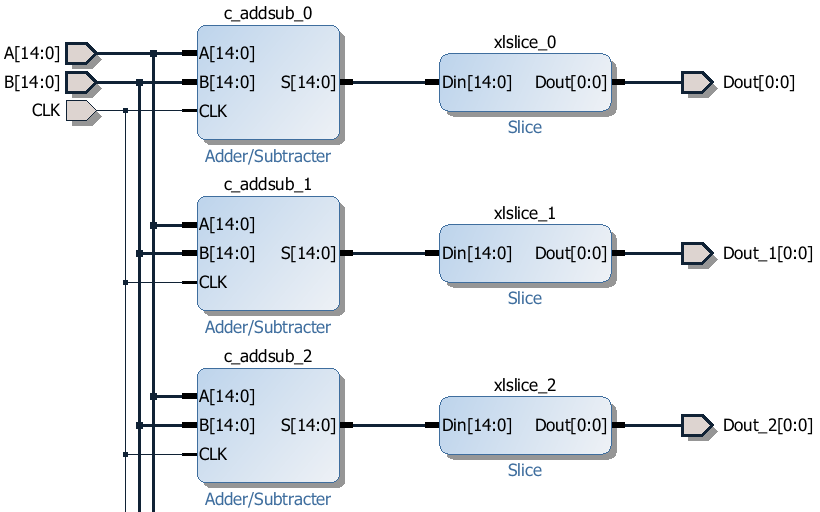
\includegraphics[width=0.75\textwidth]{figures/Blockdesignexample.png}
  \caption{Example of block design in vivado}
  \label{fig:blodesexa}
\end{figure}
The reasoning for 100 copies is to ensure that the contribution from control signals and wiring is minimized. With a block design generated it can be synthesized. In Vivado there are 2 steps. The first step is \textit{synthesize} where the software figures out which hardware is needed for the system and then the next step is \textit{implementation} where the software optimize the hardware use for the platform it is implemented on. To complete the \textit{implementation} step the design have to fit the target hardware so the design must not exceed the number of available I/O ports etc. When generating the block design IP blocks from Xilinx were used and for most FUs inputs and outputs of 16 bits were used. Each output needs to be connected to its own port and this will result in the implementation step to fail since too many I/O ports are used. Connecting the outputs to temporary signals and not using these signals will result in the \textit{implementation} step to optimize and remove all the adders since the output aren't used. Instead, a Slice IP can be used to strip every bit but MSB. This results in every block only having an output size of \SI{1}{\bit} and the I/O usage have been lowered enough for the \textit{implementation} to succeed. Then the hardware utilization can be found in the software. These values are then divided by 100 to get a rough approximation of how much hardware each functional unit requires.\\
Appendix~\vref{app:alloctest} describes more thoroughly the procedure for these tests and table~\ref{tab:utilizationofelements} shows the result.
\begin{table}[ht!]
\centering
\begin{tabular}{l | c c c c }
  \toprule
   &  LUT & FF & BRAM & DSP48 \\
  \midrule
  Adder & 15 & 15 & - & - \\
  Adder/Subtracter  & $\approx 16$ & 15 & - & - \\
  Subtract  & 15 &  15 & - & - \\
  Multiplier - LUT  & 352 &  36 & - & - \\
  Multiplier - DSP48 & - & - & - & 1 \\
  \bottomrule
\end{tabular}
\caption{Number of logic elements used in average for each FU}
\label{tab:utilizationofelements}
\end{table}

Looking at the results it is noticed that the multiplier implemented with LUT requires a lot of LUTs and FFs when compared to adder/subtracter while it only requires a single DSP if implemented using DSP48 elements. From this, it is decided that the 220 DSP48 elements should mainly be used for multiplication.

\section{Wrap-up}
The first section discusses the trade-off between platforms and which platform will be used in this project which is a Zedboard. The second section describes the specifications of the Zynq Z7020 and some additional important specification of the Zedboard. Lastly, the utilization of the hardware for different functional units using the Vivado software was analyzed. From this, it is noticed that the limited number of DSP48 elements should mainly be used for multiplications since it uses more logic elements than additions and subtractions. 